\documentclass[a4paper,10pt]{report}
\usepackage[T1]{fontenc}
\usepackage{mathptmx}
\usepackage{graphicx}
\graphicspath{ {Diagrams/} }

\title{Assignment 3.2 documentation}

\author{Péter Zaváczki\\30433}

\begin{document}

\maketitle

\section{Requirements}
Design, implement and test a distributed system that uses web services to expose the server
functionalities to its clients.

\section{Functional requirements}
Consider a distributed application called “Online Tracking System” that has a GUI which exposes the following functionalities to its users:
\begin{itemize}
    \item The application has two types of users: administrators and clients.
    \item After the login, the user is redirected to its corresponding page.
    \item If the user does not have an account, it can register and become a simple user (client)
    \item The Administrator can:
    \begin{itemize}
        \item Add/remove package. The package has the following characteristics:
        \begin{itemize}
            \item Sender – Client
            \item Receiver – Client
            \item Name
            \item Description
            \item Sender City
            \item Destination City
            \item Tracking – Boolean – initially false
        \end{itemize}
        \item Register package for tracking
        \begin{itemize}
            \item The package becomes tracked, and a route is associated to it. This route represents the path of the package to the destination, as pairs of (City, Time).
        \end{itemize}
        \item Package status updating
        \begin{itemize}
            \item A new entry (City, Time) is introduced to the route
        \end{itemize}
    \end{itemize}
    \item Each time new information about a DVD is introduced in the system the application must create automatically a text file and write the information about the DVD in it    
\end{itemize}
\begin{itemize}
    \item The Client can:
    \begin{itemize}
        \item List all its packages
        \item Search packages
        \item Package status checking
    \end{itemize}
\end{itemize}

These functionalities will be exposed as 2 web services:
\begin{itemize}
    \item WS1 – SOAP Web Service: Client Login and Register and Simple Client Operations
    \item WS2 – SOAP Web Service: Administrator Operations
\end{itemize}

\section{Implementation technologies}
\begin{itemize}
    \item Develop one SOAP Web Service in .NET and the other one in JAVA
    \item The GUI can be either WEB or Desktop and can be developed in .NET or JAVA
\end{itemize}

\section{Conceptual architecture}
This application has a complex architecture. It has two Client-Server components. One of them is the webapp, in this case the Client being the user's web browser, to which the webpages are loaded and the server is the Tomcat server to which the WAR files are deployed. The other one is the SOAP based webservice deployed on a GlassFish server.
The Simple Object Access Protocol (SOAP) uses a HTTP based protocol to model an RPC style communication. Using this is advantageous, since it allows programs that run on different OSes to communicate using the above mentioned HTTP and its XML based WSDL. At one endpoint we have an implementor of the webservice who publishes it, and at another endpoint, its client, who uses it by the stubs generated based on the published WSDL abstraction.

This can be seen on figure \ref{fig:architecture_diagram}.

\begin{figure}[h]
    \centering
    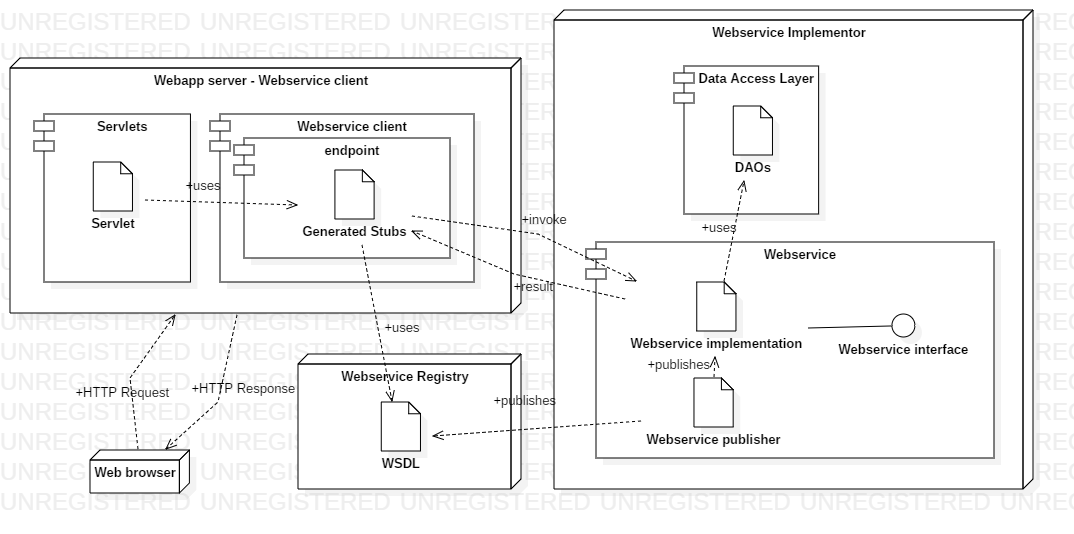
\includegraphics[width=1\textwidth]{architecture_diagram.png}
    \caption{The conceptual architecture diagram of the project}
    \label{fig:architecture_diagram}
\end{figure}

\section{Deployment}
The application is deployed on multiple nodes:
The webapp used for the UI is deployed on a Tomcat server, which has the Web Application Resource (WAR) files.
The webservice, used for SOAP based communication is deployed on a Glassfish server, and it contains information about the service in form of a WSDL file.

This deployment can be seen on figure \ref{fig:deployment_diagram}.

\begin{figure}[h]
    \centering
    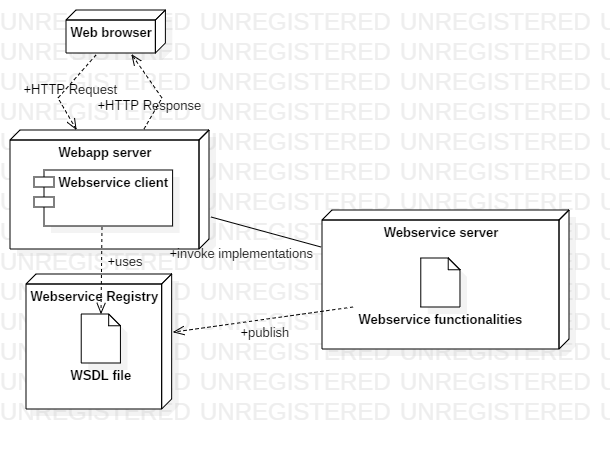
\includegraphics[width=1\textwidth]{deployment_diagram.png}
    \caption{The deployment diagram of the project}
    \label{fig:deployment_diagram}
\end{figure}

\section{Build considerations}
\begin{itemize}
    \item A web based UI was used for simplicity of development.
\end{itemize}


\end{document}
